% intro % 

\section{intro}

% check reading notes to introduce the subject.

The last type of PF particle candidates to be reconstructed are hadrons.

hadrons could start showering in the ECAL, then fully deposit their energies in HCAL.

as mentioned in previous chapter that ECAL is well calibrated for EM particles, but not for hadrons.

To accurately reconstuct these candidates, a correction for HCAL cluster energy needs to be applied after ECAL cluster calibration.

This chapter similarly to the previous one presents the used ML method and datasets in performaing the PF HCAL cluster regression.

%.................................

\section{data sets description}
we privately generate single pions samples: with  E range 2-200 GeV,200-500 GeV and under 126X conditions.
% Run3 Winter23 Digi (signle pion gun)
% since this sample is not not zero material we count the pions going throrugh the tracker ?

in this study, eta and phi of the pions are the position at the ECAL enetrance propagating through the tracker.  
we categorize particles to: 
particles that do not start a nuclear interaction in ECAL (hadronic shower) as H-hadrons.
particles that start showeing in ECAL are categorized as EH-hadrons.  

\section{PF cluster regression  using GNN}

Hadronic showers in the CMS detector have both electromagnetic and hadronic components.
These showers are not fully contained in the ECAL but extend to HCAL.

The detector response is different for EM and HAD componenets which lead to non linear energy response.
%% calorimeter response: the measurable signal produced by a calorimeter when a particle is completely absorbed within it.
%% The response of a calorimeter depends on the type of particle that is absorbed. For example, homogeneous calorimeters (like ECAL)
%% ^ are inherently nonlinear for jets and hadrons.
%% especailly for EH hadrons

The reconstructed energy of hadrons is the sum of all reconstructed hits (offline, PF reconstruct the RAW data) from the ECAL and HCAL.

Energy Reconstruction using classical  method (chi square) vs DRN (based on GNN).

Then For a given bin of ture energy
%(PF also reconstruct generated data or MC data):
by fitting the distribution of total RAW energy with Gaussian we obtain: mu and std deviation then use them to get:
Resolution (std/mu) : (which is a measure of accuracy)
and Response [(mu/E true) -1] : (which is measurement of precision) (we can see that is not linear)

%The work in this thesis is done for Run3 data.

\subsection{GNN}
GNN is a type of NN that is used to process data that can be represented as graphs.
%(explain how GNN works in a relation to the work done her)

\subsection{input features}
%(check reading notes)


loss function:  [(E true- E pre)^2/E true] %response 


\subsection{training}

%We could include the Training target.
%DRN training parameters. this include: Inpute layers (3) .. etc.
%Sample details: centrally produced GEN-SIM-RAW (two momentum range) and privately reconstructed in CMSSW.
%Rechits used as input. (we could expand more on this detail)

DRN architecture overview:
1. input: Rechits => inputNet (FCNN) *Fully Convolutional Network?*
2. => Graph Generation (KNN) => EdgeConv => calculate edge weights => graph clustering (Graclus) => graph pooling (add)
3. Global pool (max)
4. outputNet => output (E pred)
% source: PF hadron cluster calibration 26/2/2024                                                                                                                                  
%% A fully convolution network (FCN) is a neural network that only performs convolution                                                                                            
%% ^ (and subsampling or upsampling) operations. Equivalently, an FCN is a CNN without fully connected layers.                                                                      
%% ^ source: https://ai.stackexchange.com/questions/21810/what-is-a-fully-convolution-network                                                                                       
%% KNN is K-Nearest Neighbors source: https://neo4j.com/docs/graph-data-science/current/algorithms/knn/                                                                             
%% source: to understand pooling in CNN https://medium.com/@abhishekjainindore24/pooling-and-their-types-in-cnn-4a4b8a7a4611#:~:text=Global%20pooling%20reduces%20each%20channel,po\oling%20or%20global%20average%20pooling.
%% ^ in GNN https://arxiv.org/pdf/2110.05292                                                                                                                                       
%% source for node embedding https://towardsdatascience.com/node-embeddings-for-beginners-554ab1625d98    

layers:
- input 3
- aggregation 2
- output 2
- message passing2 

input:
- rechit positions
- E rechit energy corresponding to each rechit
- rechits are selected after dR matching %slide 11

batch size: 400
number of epochs trained 100
constant learning reate of 0.0001

training target:
%ratio
%ratioflip
%log (ratioflip)
%trueE

\subsection{performance and validation}
80\% of the dataset used for taining and 20\% for validation.

\section{results}
we present the results of response and resolution (from DRN vs Chi2) in  both Barrel region and endcap region.

\subsection{EH Hadrons}
the presented results are for the training target ratioflip
\begin{figure}
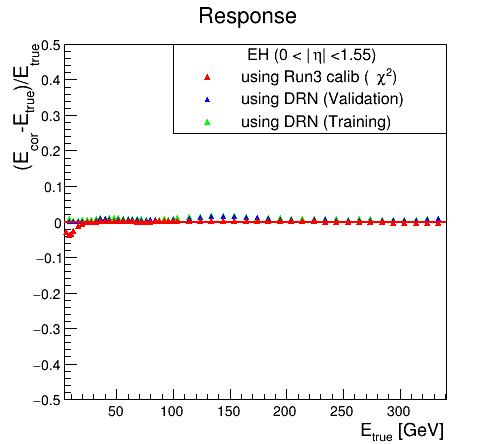
\includegraphics[width=0.495\textwidth]{./plots_pdf/HCAL_plots/Trained_target_ratioflip_0_500_10/pdf/EH_barrel/barrel_corrEtaBarrelEcalHcal.png}
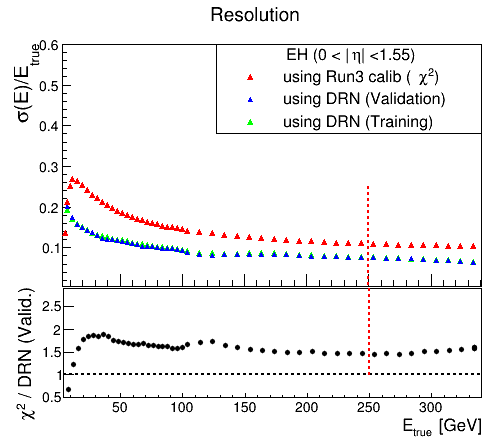
\includegraphics[width=0.495\textwidth]{./plots_pdf/HCAL_plots/Trained_target_ratioflip_0_500_10/pdf/EH_barrel/barrel_corrEtaBarrelEcalHcal_reso.png}
\caption{EH - barrel - target ratioflip}                                                                                                                                               
\end{figure}                                                                                                                                                                      

\begin{figure}                                                                                                                                                                   
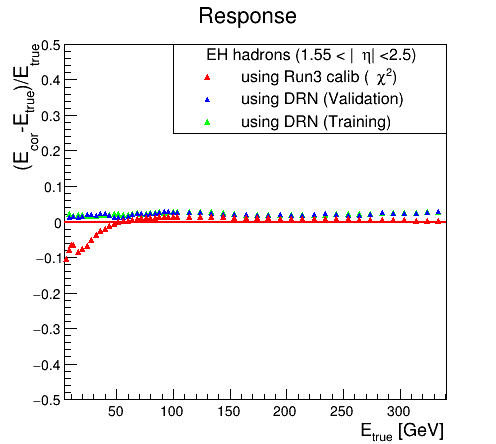
\includegraphics[width=0.495\textwidth]{./plots_pdf/HCAL_plots/Trained_target_ratioflip_0_500_10/pdf/EH_ec_in/EC_within_tracker_corrEtaEndcapEcalHcal.png}
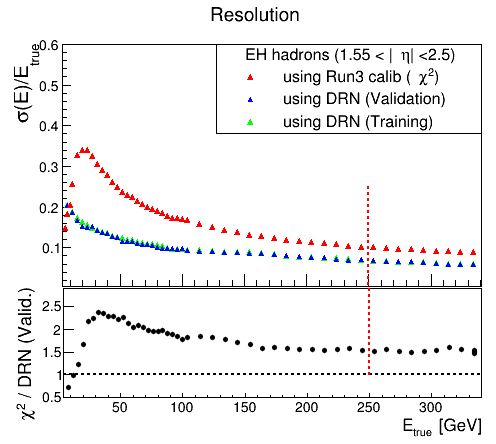
\includegraphics[width=0.495\textwidth]{./plots_pdf/HCAL_plots/Trained_target_ratioflip_0_500_10/pdf/EH_ec_in/EC_within_tracker_corrEtaEndcapEcalHcal_reso.png}
\caption{EH - endcap within tracker - target ratioflip}
\end{figure}


\begin{figure}
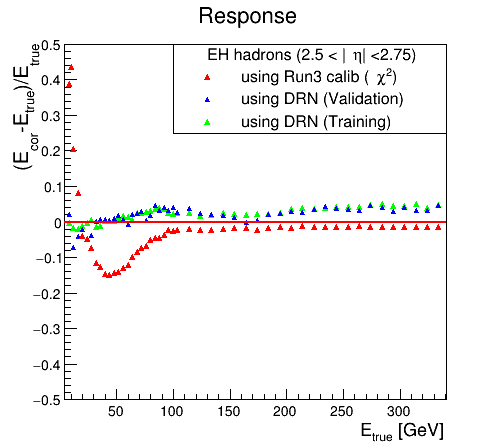
\includegraphics[width=0.495\textwidth]{./plots_pdf/HCAL_plots/Trained_target_ratioflip_0_500_10/pdf/EH_ec_out/EC_outside_tracker_corrEtaEndcapEcalHcal.png}
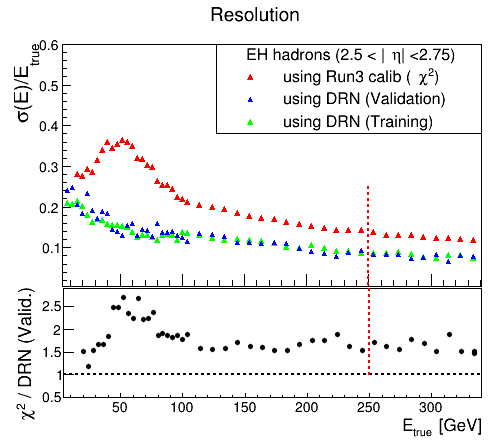
\includegraphics[width=0.495\textwidth]{./plots_pdf/HCAL_plots/Trained_target_ratioflip_0_500_10/pdf/EH_ec_out/EC_outside_tracker_corrEtaEndcapEcalHcal_reso.png}
\caption{EH - endcap outside the tracker - target ratioflip}
\end{figure}



\subsection{H hadrons}
